\chapter{إظهار صور}

لقد تعلّمنا كيف نقوم بتحميل الـ\textenglish{SDL}،
فتح نافذة و التعامل مع المساحات. إنها بالفعل من المبادئ التي تجب معرفتها عن هذه المكتبة. لكن لحدّ الآن لا يمكننا سوى إنشاء مساحات موحّدة اللون، و هذا الأمر بدائي قليلاً.

في هذا الفصل، سنتعلّم كيف نقوم بتحميل صور على مساحات، مهما كانت صيغتها
\textenglish{BMP}،
\textenglish{PNG}
أو حتى 
\textenglish{GIF}
أو 
\textenglish{JPG}.
التحكم في الصور أمر مهم للغاية لأنه بتجميع الصور (نسميها أيضاً 
"\textenglish{sprites}")
نضع اللبنات الأولى في بناء لعبة فيديو.

\section{تحميل صورة \textenglish{BMP}}

الـ\textenglish{SDL}
هي مكتبة بسيطة جداً. فهي لا تستطيع أساسا تحميل سوى صور من نوع
"\textenglish{bitmap}"
(ذات امتداد
\InlineCode{.bmp}).
لا تقلق، فبفضل إضافة خاصّة بالـ\textenglish{SDL}
(المكتبة
\textenglish{SDL\_Image})،
 سنرى بأنه بإمكاننا أيضاً تحميل صور من صيغ أخرى.
 
 للبدأ، سنكتفي الآن بما تسمح لنا به الـ\textenglish{SDL}
 بشكل قاعدي. سنقوم بدراسة تحميل صور
\textenglish{BMP}.

\subsection{الصيغة \textenglish{BMP}}

الصيغة
\textenglish{BMP}
(إختصار لـ\textenglish{bitmap})
هي صيغة صور.\\
الصور الّتي نجدها في الحاسوب مخزّنة في ملفات. يوجد العديد من صيغ الصور، أي العديد من الطرق لتخزين صورة في ملف. على حسب الصيغة، يمكن للصورة أخذ الكثير أو القليل من مساحة القرص الصلب، و تملك جودة أحسن أو أسوء.

الـ\textenglish{Bitmap}
هي صيغة غير مضغوطة (على عكس الـ\textenglish{JPG}، \textenglish{PNG}، \textenglish{GIF}،
إلخ).
فعليّا، هذا يعني الأمور التالية~:

\begin{itemize}
	\item يكون الملف سريعاً جداً من ناحية قراءته، على عكس الصيغ المضغوطة التي يجب أن يتم فك الضغط عنها، مما يكلّفنا بعض الوقت.
	\item جودة الصورة مثالية. بعض الصيغ المضغوطة (أفكّر في الـ\textenglish{JPG}
	خصوصا، لأن الـ\textenglish{PNG}
	و الـ\textenglish{GIF}
	لا يغيّرون في الصورة) تقوم بتخريب جودة الصورة، و هذا ليس هو الحال بالنسبة للـ\textenglish{BMP}.
	\item لكنّ الملف سيكون ضخماً بما أنه ليس مضغوطاً !
\end{itemize}

توجد هناك إذا مزايا و مساوئ.\\
بالنسبة للـ\textenglish{SDL}،
الشيء الجيد هو أن نوع الملف سيكون بسيطا و سهل القراءة. إذا كان عليك تحميل الصور دائما في نفس وقت تشغيل برنامجك، من المستحسن استعمال صور بصيغة 
\textenglish{BMP}.
سيكون حجم الملف ضخما حتما، لكنه يـُحمّل بشكل أسرع من الـ\textenglish{GIF}
مثلاً. سيكون الأمر مهّما إذا كان على برنامجك تحميل الكثير من الصور في وقت قليل.

\subsection{تحميل صورة \textenglish{Bitmap}}

\subsubsection{تنزيل حزمة الصور}

في هذا الفصل سنقوم بالعمل على كثير من الصور. إذا أردت القيام بتجريب الشفرات بينما أنت تقرأ (و هذا ما يجدر بك فعله !)، فأنصحك بتنزيل حزمة الصور التي تحتوي كل الصور التي نحتاج إليها.

\textenglish{\url{https://openclassrooms.com/uploads/fr/ftp/mateo21/pack_images_sdz.zip} (1 Mo)}

بالطبع، يمكنك استعمال صورك الخاصة. يجب عليك فقط أن تعدّل مقاييس النافذة على حسب مقاييس الصورة.

قم بوضع كل الصور في مجلّد المشروع. سنبدأ أولاّ بالعمل على الصورة 
\InlineCode{lac\_en\_montagne.bmp}.
هي عبارة عن لقطة تم استخلاصها من مشهد ثلاثي الأبعاد مأخوذ من البرنامج الممتاز الخاص بنمذجة المناظر الطبيعية
\textenglish{Vue d'Espri 4}،
و الذي تم إيقاف تسويقه. منذ ذلك، تمّ تغيير اسم البرنامج إلى
\textenglish{Vue}
و تم تطويره كثيراً. لمن يريد معرفة المزيد عنه، يمكنه زيارة الموقع :
\url{http://www.e-onsoftware.com/}.

\subsubsection{تحميل صورة في مساحة}

سنقوم باستعمال دالة تقوم بتحميل صورة ذات صيغة
\textenglish{BMP}
و لصقها في مساحة.\\
هذه الدالة تدعى 
\InlineCode{SDL\_LoadBMP}
و سترى أن استعمالها سهل للغاية :

\begin{Csource}
mySurface = SDL_LoadBMP("image.bmp");
\end{Csource}

الدالة
\InlineCode{SDL\_LoadBMP}
تقوم بتعويض دالتين تعرفهما :

\begin{itemize}
	\item \InlineCode{SDL\_CreateRGBSurface} :
	تقوم بحجز مكان في الذاكرة من أجل تخزين مساحة ذات الحجم المطلوب (تكافئ دالة 
	\InlineCode{malloc}).
	\item \InlineCode{SDL\_FillRect} :
	تقوم بملئ الهيكل بلون موحّد.
\end{itemize}
لماذا تقوم الدالة بتعويض هذين الدالتين ؟ الأمر بسيط :
\begin{itemize}
	\item الحجم الذي نقوم بحجزه في الذاكرة  من أجل المساحة يعتمد على حجم الصورة : اذا كان حجم الصورة هو 
	$250 \times 300$
	فستأخذ المساحة نفس الحجم.
	\item من جهة أخرى، يتم ملئ المساحة بيكسلا ببيكسل بمحتوى الصورة 
	\textenglish{BMP}.
\end{itemize}

فلنكتب الشفرة دون أي تأخير :

\begin{Csource}
int main(int argc, char *argv[])
{
	SDL_Surface *screen = NULL, *backgroundImage = NULL;
	SDL_Rect backgroundPosition;
	backgroundPosition.x = 0;
	backgroundPosition.y = 0;
	SDL_Init(SDL_INIT_VIDEO);
	screen = SDL_SetVideoMode(800, 600, 32, SDL_HWSURFACE);
	SDL_WM_SetCaption("Loading the images on SDL", NULL);
	/* Loading a Bitmap image in a surface */	
	backgroundImage = SDL_LoadBMP("lac_en_montagne.bmp");
	/* We blit on the screen */
	SDL_BlitSurface(backgroundImage, NULL, ecran, &backgroundPosition);
	SDL_Flip(screen);
	pause();
	SDL_FreeSurface(backgroundImage); // We free the surface
	SDL_Quit();
	return EXIT_SUCCESS;
}
\end{Csource}

و بهذا أكون قد أنشأت مؤشّراً نحو مساحة
(\InlineCode{backgroundImage})
و نحو كل المركّبات الموافقة لها
(\InlineCode{backgroundPosition}).\\
تم إنشاء المساحة في الذاكرة و ملؤها من طرف الدالة 
\InlineCode{SDL\_LoadBMP}.\\
نقوم بتسويتها على المساحة 
\InlineCode{screen}
و هذا كلّ شيء ! الصورة التالية توضّح النتيجة :

\Picture{Chapter_III-3_Window-Image}

كما ترى، لم يكن الأمر صعباً !

\subsubsection{إرفاق أيقونة بالتطبيق}

بما أننا الآن نجيد تحميل الصور، يمكننا اكتشاف كيفية إرفاق أيقونة بالبرنامج. سيتم إظهار الأيقونة في أعلى يسار النافذة (و أيضاً في شريط المهام). لحدّ الآن نحن لا نملك إلاّ أيقونة افتراضيّة.

\begin{question}
لكن ألا يجدر بأيقونات البرامج أن تكون ذات الامتداد
\InlineCode{.ico} ؟
\end{question}

كلّا، ليس شرطاً ! على كلّ فالامتداد
\InlineCode{.ico}
لا يوجد إلا في نظام الويندوز. الـ\textenglish{SDL}
تتعامل مع كلّ أنظمة التشغيل باستعمالها نظاما خاصا بها : المساحة !\\
نعم، أيقونة برنامج 
\textenglish{SDL}
ماهي إلا مساحة بسيطة.

\begin{warning}
يجدر بالأيقونة أن تكون ذات حجم 
$16 \times 16$
بيكسلز. بينما في الويندوز يجب أن تكون بحجم
$32 \times 32$
بيكسلز و إلا فستسوء جودتها. لا تقلق إذ يمكن للـ\textenglish{SDL}
"تصغير" أبعاد الصورة لتتمكن من الدخول في 
$16 \times 16$
بيكسلز.
\end{warning}

لإضافة الأيقونة إلى النافذة، نستعمل الدالة 
\InlineCode{SDL\_WM\_SetIcon}.\\
هذه الدالة تأخذ معاملين : المساحة التي تحتوي الصورة التي نريد إظهارها كما أنها تستقبل معلومات حول الشفافية (القيمة 
\InlineCode{NULL}
تعني أننا لا نريد أية شفافية). التحكّم في الشفافية الخاصة بأيقونة معقّد قليلاً (يجب تحديد البيكسلز الشفافة واحدة بواحدة)، لن ندرس ذلك إذا.

سنقوم باستدعاء دالة في استدعاء لأخرى :

\begin{Csource}
SDL_WM_SetIcon(SDL_LoadBMP("sdl_icone.bmp"), NULL);
\end{Csource}
 
تم تحميل الصورة في الذاكرة بواسطة
\InlineCode{SDL\_LoadBMP}
و تم بعث عنوان المساحة مباشرة إلى
\InlineCode{SDL\_WM\_SetIcon}.

\begin{critical}
يجب أن يتم استدعاء الدالة
\InlineCode{SDL\_WM\_SetIcon}
قبل أن يتم فتح النافذة، أي أنه يجدر بها التواجد قبل
\InlineCode{SDL\_SetVideoMode}
في الشفرة المصدرية.
\end{critical}

هذه هي الشفرة المصدرية الكاملة. ستلاحظ أنني أضفت
\InlineCode{SDL\_WM\_SetIcon}
مقارنة بالشفرة السابقة.

\begin{Csource}
int main(int argc, char *argv[])
{
	SDL_Surface *screen = NULL, *backgroundImage = NULL;
	SDL_Rect backgroundPosition;
	backgroundPosition.x = 0;
	backgroundPosition.y = 0;
	SDL_Init(SDL_INIT_VIDEO);
	/* Loading the icon before SDL_SetVideoMode*/
	SDL_WM_SetIcon(SDL_LoadBMP("sdl_icone.bmp"), NULL);
	screen = SDL_SetVideoMode(800, 600, 32, SDL_HWSURFACE);
	SDL_WM_SetCaption("Loading images on SDL", NULL);
	backgroundImage = SDL_LoadBMP("lac_en_montagne.bmp");
	SDL_BlitSurface(backgroundImage, NULL, screen, &backgroundPosition);
	SDL_Flip(screen);
	pause();
	SDL_FreeSurface(backgroundImage);
	SDL_Quit();
	return EXIT_SUCCESS;
}
\end{Csource}

النتيجة : تم تحميل الصورة و عرضها أعلى يسار النافذة.
\Picture{Chapter_III-3_Window-icon}

\section{التحكم في الشفافية}

\subsection{مشكل الشفافية}

لقد قمنا قبل قليل بتحميل صورة 
\textenglish{bitmap}
في النافذة.\\
لنفرض أننا نريد لصق صورة فوقها. و هذا ما يحصل كثيراً في الألعاب. غالبا اللاعب الذي يتحرّك في الخريطة هو عبارة عن صورة 
\textenglish{bitmap}
تتحرك فوق صورة خلفية.

سنقوم بلصق صورة
\textenglish{Zozor}
(لمن لا يعرفه، فهو شعار
\textenglish{Site du Zéro}
سلف الموقع 
\textenglish{OpenClassrooms}
حاليّا) في المشهد :

\begin{Csource}
int main(int argc, char *argv[])
{
	SDL_Surface *screen = NULL, *backgroundImage = NULL, *zozor = NULL;
	SDL_Rect backgroundPosition, zozorPosition;
	backgroundPosition.x = 0;
	backgroundPosition.y = 0;
	zozorPosition.x = 500;
	zozorPosition.y = 260;
	SDL_Init(SDL_INIT_VIDEO);
	SDL_WM_SetIcon(SDL_LoadBMP("sdl_icone.bmp"), NULL);
	screen = SDL_SetVideoMode(800, 600, 32, SDL_HWSURFACE);
	SDL_WM_SetCaption("Loading images on SDL", NULL);
	backgroundImage = SDL_LoadBMP("lac_en_montagne.bmp");
	SDL_BlitSurface(backgroundImage, NULL, ecran, &backgroundPosition);
	//Loading and blitting Zozor on the screen
	zozor = SDL_LoadBMP("zozor.bmp");
	SDL_BlitSurface(zozor, NULL, screen, &zozorPosition);
	SDL_Flip(screen);
	pause();
	SDL_FreeSurface(backgroundImage);
	SDL_FreeSurface(zozor);
	SDL_Quit();
	return EXIT_SUCCESS;
}
\end{Csource}

لقد قمنا فقط بإضافة مساحة لنخزّن فيها 
\textenglish{Zozor}،
و التي نقوم بلصقها في مكان معيّن من المشهد :

\Picture{Chapter_III-3_Window-Image-Zozor}

يبدو المشهد سيّئا، أليس كذلك ؟

\begin{question}
بالطبع يعود ذلك إلى الخلفية الزرقاء التي هي خلف 
\textenglish{Zozor} !
\end{question}

لأنك تعتقد أنه بوجود خلفية سوداء أو بنّيّة، ربما سيكون المظهر لائقاً أكثر ؟ لا بالطبع، المشكل هنا هو أنه من اللازم أن يكون شكل الصورة عبارة عن مستطيل، أي أنه إذا قمنا بلصقها على المشهد، سنرى خلفيتها، مما يشوّه المظهر.

من حسن الحظّ أن الـ\textenglish{SDL}
تتحكم في الشفافية !

\subsection{جعل صورة شفافة}

\subsubsection{الخطوة 1 : تحضير الصورة}

كبداية، يجب تحضير الصورة التي نريد تسويتها على المشهد.\\
الصيغة 
\textenglish{BMP}
لا تتحكم في الشفافية، على عكس الصيغتين 
\textenglish{GIF}
و 
\textenglish{PNG}.
لهذا يحب علينا أن نجد حلاً آخر. 

يجب استعمال نفس اللون للخلفية على الصورة. هذه الأخيرة ستكون شفافة من طرف الـ\textenglish{SDL}
في وقت التسوية. لاحظ كيف تبدو الصورة
\InlineCode{zozor.bmp}
من ناحية أقرب :

\Picture{Chapter_III-3_Zozor}

الخلفية الزرقاء إذا مـُختارة. لاحظ أنني اخترت اللون الأزرق بشكل عشوائي، كان بإمكاني استعمال اللون الأحمر أو الأصفر مثلاً. الشيء المهم هو أنه يجب على اللون أن يكون وحيداً و موحّدا. لقد اخترت اللون الأزرق لأنه ليس متواجدا في صورة 
\textenglish{Zozor}
لأنني لو اخترت اللون الأخضر، سأخاطر بجعل العشب الذي يتناوله الحمار (أسفل يسار الصورة) شفافاً. 

استعمل إذا أي برنامج كان 
(\textenglish{Paint}، \textenglish{Photoshop}، \textenglish{The Gimp}، \dots
لكلّ واحد منّا ذوقه) لإعطاء خلفية موحّدة للصورة.

\subsubsection{الخطوة 2 : تحديد اللون الشفاف}

لكي نقوم بتحديد اللون الذي يجب أن تجعله
\textenglish{SDL}
شفافاً، يجب أن نستعمل الدالة 
\InlineCode{SDL\_SetColorKey}.
يجب استدعاء هذه الدالة قبل تسوية الصورة.\\
هكذا نقوم بتحويل اللون الذي خلف
\textenglish{Zozor}
إلى الشفاف :

\begin{Csource}
SDL_SetColorKey(zozor, SDL_SRCCOLORKEY, SDL_MapRGB(zozor->format, 0, 0, 255));
\end{Csource}

هناك ثلاثة معاملات :

\begin{itemize}
	\item المساحة التي يجب أن نقوم بتحويلها إلى اللون الشفاف (هنا نتكلم عن 
	\InlineCode{zozor}).
	\item قائمة الأعلام : استعمل 
	\InlineCode{SDL\_SRCCOLORKEY}
	لتفعيل الشفافية، 0 من أجل تعطيلها.
	\item حدد بعد ذلك اللون الذي يجب أن يتم تحويله إلى الشفاف. لقد استعملت
	\InlineCode{SDL\_MapRGB}
	لإنشاء اللون بصيغة عدد
	(\InlineCode{Uint32})
	كما فعلنا بالسابق. كما ترى إنه اللون الأزرق 
	($0, 0, 255$)
	 الّذي سيتم تحويله إلى الشفاف.
	
\end{itemize}

كملخص، نقوم أولا بتحميل الصورة باستعمال
\InlineCode{SDL\_LoadBMP}،
ثمّ نحدد اللون الشفاف باستعمال
\InlineCode{SDL\_SetColorKey}
ثم نقوم بتسوية المساحة باستعمال
\InlineCode{SDL\_BlitSurface}.

\begin{Csource}
zozor = SDL_LoadBMP("zozor.bmp");
SDL_SetColorKey(zozor, SDL_SRCCOLORKEY, SDL_MapRGB(zozor->format, 0, 0, 255));
SDL_BlitSurface(zozor, NULL, screen, &zozorPosition);
\end{Csource}

النتيجة : تم دمج صورة
\textenglish{Zozor}
بشكل ممتاز في المشهد :

\Picture{Chapter_III-3_Window-Image-Zozor-transparent}

هذه هي التقنية المبدئية التي ستعيد استعمالها كل الوقت في برامجك. تعلّم كيف تتحكم جيداً بالشفافية لأنها من أساسيات صنع لعبة تملك الحدّ الأدنى من الواقعية.

\subsection{الشفافية \textenglish{Alpha}}

هو نوع آخر من الشفافية.\\
لحدّ الآن قمنا بتعريف لون 
\underline{واحد}
شفاف (الأزرق مثلا). هذا اللون لا يظهر في الصورة المُلصقة. 

الشفافية 
\textenglish{Alpha}
توافق شيئاً آخر، إنها تسمح بعمل "مزج" بين صورة و خلفية. هذا نوع من التلاشي.

يمكن تفعيل الشفافية
\textenglish{Alpha}
لمساحة عن طريق الدالة
\InlineCode{SDL\_SetAlpha} :

\begin{Csource}
SDL_SetAlpha(zozor, SDL_SRCALPHA, 128);
\end{Csource}

يوجد هنا ثلاثة معاملات كذلك :

\begin{itemize}
	\item المساحة التي نتكلم عنها (\InlineCode{zozor}).
	\item قائمة الأعلام : ضع
	\InlineCode{SDL\_SRCALPHA}
من أجل تفعيل الشفافية، 0 من أجل تعطيلها.
	\item مهم جدا : قيمة الشفافية 
\textenglish{Alpha}
هي عدد يتراوح بين 0 (صورة شفافة تماماً أي غير مرئية) و 255 (صورة ظاهرة كلياً، و كأن الشفافية
\textenglish{Alpha}
لم تكن موجودة).
\end{itemize}

كلما كان العدد
\textenglish{Alpha}
صغيراً كلما زادت شفافية الصورة و تلاشيها في الخلفية.

هذا مثال عن شفرة تقوم بتطبيق شفافية بقيمة 128 على الصورة
\textenglish{Zozor} :

\begin{Csource}
zozor = SDL_LoadBMP("zozor.bmp");
SDL_SetColorKey(zozor, SDL_SRCCOLORKEY, SDL_MapRGB(zozor->format, 0, 0, 255));
/* Average Alpha transparency (128) : */
SDL_SetAlpha(zozor, SDL_SRCALPHA, 128);
SDL_BlitSurface(zozor, NULL, screen, &zozorPosition);
\end{Csource}

تلاحظ أنني حافظت على شفافية 
\InlineCode{SDL\_SetColorKey}.
يمكن دمج النوعين الاثنين للشفافية معاً.

الجدول التالي يوضّح لك كيف يبدو
\textenglish{Zozor}
باختلاف قيم
\textenglish{Alpha}.

\begin{Table}{2}
\textenglish{Alpha} & النتيجة\\
255 (مرئيّة بالكامل) &
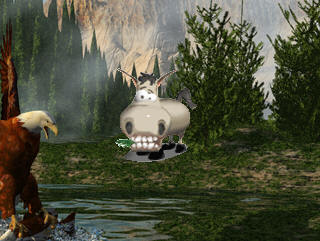
\includegraphics[width=0.25\textwidth]{Chapter_III-3_Window-Image-Zozor-Alpha-255} \\
190 &
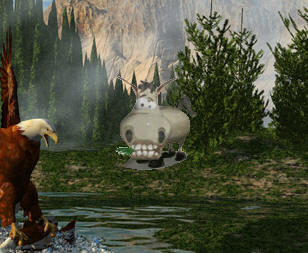
\includegraphics[width=0.25\textwidth]{Chapter_III-3_Window-Image-Zozor-Alpha-190} \\
128 (شفافيّة متوسّطة) &
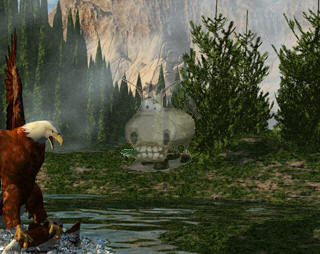
\includegraphics[width=0.25\textwidth]{Chapter_III-3_Window-Image-Zozor-Alpha-128} \\
75 &
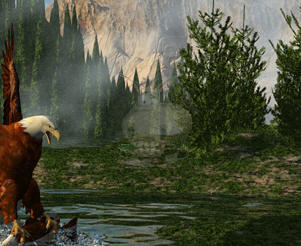
\includegraphics[width=0.25\textwidth]{Chapter_III-3_Window-Image-Zozor-Alpha-75} \\
\end{Table}
\begin{Table*}{2}
0 (غير مرئيّة بالكامل) &
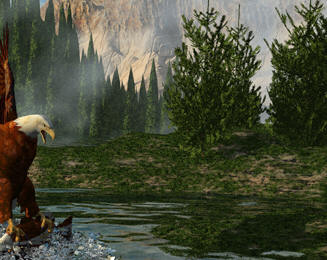
\includegraphics[width=0.25\textwidth]{Chapter_III-3_Window-Image-Zozor-Alpha-0} \\
\end{Table*}


\begin{information}
قيمة الشفافية
\textenglish{Alpha}
128 (شفافية متوسطة) هي قيمة خاصّة و كثيرة الإستعمال بالـ\textenglish{SDL}.
هذا النمط من الشفافية أسرع من ناحية حسابات المعالج مقارنة بالأنماط الأخرى. قد يكون من المهم لك معرفة هذه المعلومة خاصة إن كنت تستعمل الشفافية
\textenglish{Alpha}
بشكل كبير في برامجك.
\end{information}

\section{تحميل صيغ صور أخرى باستعمال الـ\textenglish{SDL\_Image}}

الـ\textenglish{SDL}
لا تتعامل إلا مع الـ\textenglish{bitmap}
(الصيغة
\textenglish{BMP})
كما رأينا.\\
و لكن هذا ليس بمشكل لأن قراءة الصور ذات الصيغة 
\textenglish{BMP}
أسرع بالنسبة للـ\textenglish{SDL}،
و لكن يجب معرفة أنه في أيامنا هذه يتم استعمال صيغ أخرى للصور. بالتحديد الصيغ "المضغوطة" كالـ\textenglish{PNG}،
الـ\textenglish{GIF}
و الـ\textenglish{JPEG}.
لهذا الغرض توجد مكتبة تسمى
\textenglish{SDL\_Image}
و تقوم بالتعامل مع كل صيغ الصور التالية :

\begin{itemize}
	\item \textenglish{TGA}،
	\item \textenglish{BMP}،
	\item \textenglish{PNM}،
	\item \textenglish{XPM}،
	\item \textenglish{XCF}،
	\item \textenglish{PCX}،
	\item \textenglish{GIF}،
	\item \textenglish{JPG}،
	\item \textenglish{TIF}،
	\item \textenglish{LBM}،
	\item \textenglish{PNG}.
\end{itemize}

بالمناسبة فإنه بالإمكان أن تتم إضافة صيغ أخرى للـ\textenglish{SDL}.
و هي المكتبات التي تحتاج إلى الـ\textenglish{SDL}
لكي تعمل. يمكننا تسمية هذا الأمر بالـ\textenglish{add-ons}
(بمعنى "إضافات").
\textenglish{SDL\_Image}
هي واحدة من بين هذه المكتبات .

\subsection{تثبيت الـ\textenglish{SDL\_Image} على \textenglish{Windows}}

\subsubsection{التنزيل}

توجد صفحة خاصة من موقع الـ\textenglish{SDL}
تشير إلى المكتبات التي تستعملها الـ\textenglish{SDL}.
هذه الصفحة تحمل عنوان
"\textenglish{Libraries}".
ستجد رابطاً في القائمة اليسارية.\\
ستلاحظ أن هناك الكثير من المكتبات و أغلبها ليس من طرف المبرمجين الأصليين للـ\textenglish{SDL}.
بل هم مبرمجون عاديون يستعملون الـ\textenglish{SDL}
و يقومون باقتراح مكتباتهم الخاصة لتحسين هذه الأخيرة.

بعض هذه المكتبات مفيد جداً و يستحق إلقاء النظر عليه، و بعضها أقلّ جودة بل ربّما فيه أخطاء. لهذا يجب ترتيب هذه المكتبات حسب أهميتها.

حاول إيجاد
\textenglish{SDL\_Image}
في القائمة، ستدخل إلى الصفحة المخصصة لهذه المكتبة :

\url{https://www.libsdl.org/projects/SDL_image}

حمّل النسخة التي تناسبك من القسم
"\textenglish{Binary}"
(لا تحمّل الملفات المصدرية، لن نحتاجها !).\\
إذا كنت تعمل على الويندوز، حمّل الملف
\InlineCode{SDL\_image-devel-1.2.10-VC.zip}،
و هذا حتى و إن لم تكن تستعمل البيئة التطويرية 
\textenglish{Visual C++} !

\subsubsection{التثبيت}

في الملف
\InlineCode{.zip}
هذا، ستجد :

\begin{itemize}
	\item \InlineCode{SDL\_image.h} :
	 الملف الرأسي الوحيد الذي تحتاجه الـ\textenglish{SDL\_Image}،
	 قم بلصقه في المسار
	 
	 \InlineCode{C:\textbackslash Program Files\textbackslash CodeBlocks\textbackslash SDL-1.2.13\textbackslash include}
	 
	 بمعنى آخر، إلى جانب الملفات الرأسية للـ\textenglish{SDL}.
	\item \InlineCode{SDL\_image.lib} :
	قم بلصقه في المسار
	
	\InlineCode{C:\textbackslash Program Files\textbackslash CodeBlocks\textbackslash SDL-1.2.13\textbackslash lib}.
	
	أعرف أنك ستخبرني بأن الملفات ذات الامتداد
	\InlineCode{.lib}
	هي محجوزة للبيئة التطويرية
	\textenglish{Visual C++}،
	لكن هذه حالة استثنائية، فالملف 
	\InlineCode{.lib}
	يعمل حتى مع المترجم 
	\textenglish{mingw}.
	\item الكثير من الملفات
	\textenglish{DLL} : 
	قم بوضعها كلها في المجلّد الخاص بالمشروع (أي بجانب الملف 
	\InlineCode{SDL.dll}).
\end{itemize}

بعد ذلك، يجدر بك تغيير خواص المشروع من أجل محرّر الروابط
(\textenglish{Linker})
للملف
\InlineCode{SDL\_image.lib}.

إذا كنت تعمل بالـ\textenglish{Code::Blocks}
مثلاً، توجّه إلى القائمة
\InlineCode{Projects} / \InlineCode{Build options}،
في الفرع
\InlineCode{Linker}
أنقر على الزر 
\InlineCode{Add}
و اختر المسار الذي يتواجد به الملف
\InlineCode{SDL\_image.lib}،
لاحظ الصورة :

\Picture{Chapter_III-3_CodeBlocks-Linker}

إذا ظهرت لك رسالة تحمل سؤال : 
"\textit{\textenglish{Keep as a relative path ?}}"،
فلتجب بما أردت لأنه لن يغير شيئاً في الوقت الحالي. أنصحك بالإجابة بالسلب، شخصيّا.

بعد ذلك، ما عليك سوى تضمين الملف الرأسي
\InlineCode{SDL\_image.h}
في الشفرة المصدرية. على حسب المكان الذي وضعت فيه الملف
\InlineCode{SDL\_image.h}
سيكون عليك استعمال هذه الشفرة :

\begin{Csource}
#include <SDL/SDL_image.h>
\end{Csource}

أو هذه

\begin{Csource}
#include <SDL_image.h>
\end{Csource}

جرّبهما كليهما، يجدر بأحداهما أن تعمل.

\begin{information}
إذا كنت تعمل بالـ\textenglish{Visual Studio}
فستكون العمليّة نفسها. لأنه إن تمكنت من تثبيت الـ\textenglish{SDL}
لن يصعب عليك تثبيت الـ\textenglish{SDL\_Image}.
\end{information}

\subsection{تثبيت الـ\textenglish{SDL\_Image} على \textenglish{Mac OS X}}


إن كنت تستعمل
\textenglish{Mac OS X}،
نزّل الملف ذو الامتداد
\InlineCode{.dmg}
من موقع الـ\textenglish{SDL}
و ضعه في المجلد\\
\InlineCode{Library/Frameworks}.

اكتب بعد ذلك
"\textenglish{search paths}"
 في حقل البحث الخاص بـ\textenglish{Xcode}.
 اعثر على السطر\\
\InlineCode{Header search paths}،
 انقر مرتين على السطر من اليمين و أضف\\
\InlineCode{/Library/Frameworks/SDL\_image.framework/Headers}.

لم يبق لك سوى اضافة إطار العمل إلى المشروع. الصورة التالية توضح لك كيف يظهر\\
الـ\InlineCode{Header search paths}
بعد تثبيت الـ\textenglish{SDL\_image}.

\Picture{Chapter_III-3_Xcode-frameworks}

و بهذا يجب عليك تضمين الملف الرأسي في بداية الكود كالتالي :
\begin{Csource}
#include "SDL_image.h"
\end{Csource}
في عوض استعمال الإشارتين
\InlineCode{< >}
 قم باستعمال الكتابة السابقة فيما سأعطيك لاحقا.

\subsection{تحميل الصور}

الحقيقة أن تثبيت الـ\textenglish{SDL\_image}
أصعب بمئة مرة من استعمالها ! إنه عليك أنت تحديد صعوبة العمل بالمكتبة~! 

توجد دالة وحيدة عليك معرفتها : 
\InlineCode{IMG\_Load}.\\
و هي تستقبل معاملا واحدا : اسم الملف الذي نريد فتحه.

و هذا أمر عملي لأن هذه الدالة تتمكن من تحميل أي نوع من الملفات التي تتعامل معهاالـ\textenglish{SDL\_image}
(\textenglish{JPG}، \textenglish{PNG}، \textenglish{GIF}
و حتى الـ\textenglish{TIF}،
إلخ). إذ تقوم وحدها بتحديد نوع الملف من خلال امتداده.
\begin{question}
بما أن الـ\textenglish{SDL\_Image}
تستطيع أيضاً فتح الصور 
\textenglish{BMP}،
فيمكنك الآن نسيان أمر استعمال الدالة 
\InlineCode{SDL\_LoadBMP}
و استعمال الدالة 
\InlineCode{IMG\_Load}
لتحميل كل أنواع الصور.
\end{question}

شيء جيد آخر : إذا كانت الصورة التي تحمّلها تملك الشفافية (كما هو حال الصور 
\textenglish{PNG}
و
\textenglish{GIF})
 فإنّ
\textenglish{SDL\_Image}
تفعّل تلقائيّا الشفافية من أجل هذه الصورة ! مما يعني عدم وجود داعٍ لاستدعاء الدالة 
\InlineCode{SDL\_SetColorKey}.

سأٌقدّم لك الشفرة المصدرية التي تقوم بتحميل الصورة 
\InlineCode{sapin.png}
و إظهارها.\\
لاحظ جيدا أنني قمت بتضمين
\InlineCode{SDL/SDL\_image.h}
كما أنني لا استدعي الدالة 
\InlineCode{SDL\_SetColorKey}
لأن الصورة
\textenglish{PNG}
التي استعملها شفافة طبيعيّا.\\
سترى أنني أستعمل الدالة 
\InlineCode{IMG\_Load}
في كلّ مكان بالشفرة و ذلك بتعويض الدالة 
\InlineCode{SDL\_LoadBMP}.

\begin{Csource}
#include <stdlib.h>
#include <stdio.h>
#include <SDL/SDL.h>
/* including the header of SDL_image (adapt your directory) */
#include <SDL/SDL_image.h> 
void pause();
int main(int argc, char *argv[])
{
	SDL_Surface *screen = NULL, *backgoundImage = NULL, *sapin = NULL;
	SDL_Rect backgoundPosition, sapinPosition;
	backgoundPosition.x = 0;
	backgoundPosition.y = 0;
	sapinPosition.x = 500;
	sapinPosition.y = 260;
	SDL_Init(SDL_INIT_VIDEO);
	SDL_WM_SetIcon(IMG_Load("sdl_icone.bmp"), NULL);
	screen = SDL_SetVideoMode(800, 600, 32, SDL_HWSURFACE);
	SDL_WM_SetCaption("Loading images on SDL", NULL);
	backgoundImage = IMG_Load("lac_en_montagne.bmp");
	SDL_BlitSurface(backgoundImage, NULL, screen, &backgoundPosition);
	/* Loading a PNG image with IMG_Load
	We won't have any problem because the PNG image contains the transparency information inside */
	sapin = IMG_Load("sapin.png");
	SDL_BlitSurface(sapin, NULL, screen, &sapinPosition); 
	SDL_Flip(screen);
	pause();
	SDL_FreeSurface(backgroundImage);
	SDL_FreeSurface(sapin);
	SDL_Quit();
	return EXIT_SUCCESS;
} 
void pause()
{
	int cont = 1;
	SDL_Event event;
	while (cont)
	{
		SDL_WaitEvent(&event);
		switch(event.type)
		{
			case SDL_QUIT:
			cont = 0;
		}
	}
}
\end{Csource}

كما يمكننا الملاحظة، فقد تم دمج الصورة مع الخلفية بشكل ممتاز :

\Picture{Chapter_III-3_Window-Image-Sapin}

\section*{ملخّص}

\begin{itemize}
	\item تسمح الـ\textenglish{SDL}
	بتحميل صور على مساحات. افتراضيّا، هي تسمح بالتعامل مع الصور ذات الصيغة
	\textenglish{BMP}
	باستعمال الدالة
	\InlineCode{SDL\_LoadBMP}.
	\item يمكننا تعريف لون شفاف باستعمال الدالة
	\InlineCode{SDL\_SetColorKey}.
	\item يمكننا جعل الصورة أكثر أو أقل شفافية و ذلك باستعمال الدالة 
	\InlineCode{SDL\_SetAlpha}.
	\item المكتبة
	\textenglish{SDL\_image}
	تسمح بإدخال صور من أيّة صيغة كانت
	(\textenglish{JPG}، \textenglish{PNG}، \dots)
	باستعمال الدالة
	\InlineCode{IMG\_Load}.
	لكن علينا تسطيب هذه المكتبة بالإضافة إلى الـ\textenglish{SDL}.
\end{itemize}
